After the first parts of the algorithm (file reading, file writing and error handling) were finished, a shell script was made to run the algorithm through every instance obtained from
\url{<https://www.mech.kuleuven.be/en/cib/op#section-14>}, so that thorough testing could be made with each increment in the algorithm's development. Before development of each phase started, the vertex and trip structures were created along with the functions that interact with them, so that any errors that could potentially disrupt data consistency would be contained and handled correctly before it could cause any havoc.

Finally, a python script was developed to plot each vertex given by the instance and the tour constructed by the algorithm, to visually see that it was working properly and as optimally as possible. Apart from this, some utility functions where created in the file $user\_io.c$ to print certain parts of the algorithm, like a trip's route or each vertices' location. After all of this was done, development on the actual algorithm started.

Before, during and after each phase described in the last section was developed, the program was tested with all instances and with different seeds, to assert that it was constantly functioning properly. Apart from this, the program was also debugged using the \textbf{Valgrind} tool to assert that memory was always being handled correctly.

A problem that appeared during the tour Greedy Randomized Construction phase was that for some instances of the problem none or only a small amount of viable solutions could be found. Due to the difficulty linked to designing an algorithm to repair these solutions while retaining good enough potential collected score, the invalid solutions were scraped at generation and the instances where no solutions could be found were scrapped.

After the algorithm's development finished, exhaustive testing was made with different values for each parameter by using the shell script mentioned before. The following conclusions were made by these tests regarding the parameters, along with a description of each:
\begin{itemize}
    \item \textbf{h\_rcl\_size}: As long as the \textbf{p\_rcl\_size} is kept between $5$ and $7$, \textbf{h\_rcl\_size} does not effect the results obtained greatly, as long as it's not $1$, which would make the hotel choice completely greedy. Values over $4$ are favoured tho, with $27$ out of the $32$ best-performing executions setting this parameter between $4$ and $10$. The default value was set to $9$, offering high exploration of wildly different solutions instead of stagnant exploitation of the same solutions over and over.
    \item \textbf{p\_rcl\_size}: As said before, values between $5$ and $7$ maximize the score collected by each solution, with $23$ out of the $32$ best-performing executions setting this parameter in that range. Due to the general size of the instances, this conclusion is logical, being a good enough point favoring exploration and exploitation equally. The default value was set to $5$, which accumulated the most best-performing executions ($9$ out of $32$) and being in the ``golden range'' described earlier.
    \item \textbf{ls\_iters\_n}: The average score collected by each tour was calculated for different values of this parameter, and this, along with the computation times, was used to set the default value to $15$, as the improvements after this value were less than $0.001\%$ and the increase in the computation time was no longer justified.
    \item \textbf{iters\_n}: As with \textbf{ls\_iter\_n}, the average score collected by each tour was calculated and was used alongside the computation times to decide on a default value, which was set at $5000$, since the improvements after this value were less than $2\%$ and the increase in the computation time was no longer acceptable.
\end{itemize}
The tests regarding \textbf{h\_rcl\_size} and \textbf{p\_rcl\_size} were made using an \textbf{iters\_n} of 100 and a \textbf{ls\_iters\_n} of 20, to be able to test with a relatively good speed, averaging out at $32103 [ms]$ for the compilation of the program and running on all the $405$ instances. Not much relation between the computation times and these values was perceived. Values for both parameters were tested between $1$ and $10$, going through each combination of the two parameters thorough this range. It is worth noting that the best performing combination of the two were $7$ for the hotel RCL and $5$ for the POI RCL.

After testing for the RCL sizes, the number of iterations for the Local Search phase were tested, keeping all the other parameters constant at 100 iterations and the RCL sizes set to the default values described before. Naturally, the value effects computation times significantly, shifting from $8203 [ms]$ when one iteration is used, to $125163 [ms]$ when a hundred iterations are used. The values for each \textbf{ls\_iters\_n} tested are shown in Table 3.

\begin{center}
    \begin{table}[]
    \centering
    \begin{tabular}{|r|r|r|}
        \hline
        \textbf{ls\_iter\_n} & impr. (\%) & comp. time [s] \\
        \hline
        $0$   & -       &   $6.968$ \\
        $1$   & $66.81$ &   $8.203$ \\
        $2$   & $7.95$  &   $9.685$ \\
        $3$   & $5.58$  &  $10.866$ \\
        $4$   & $3.57$  &  $12.127$ \\
        $5$   & $2.32$  &  $13.460$ \\
        $6$   & $1.26$  &  $14.933$ \\
        $7$   & $0.70$  &  $15.865$ \\
        $8$   & $0.34$  &  $17.223$ \\
        $9$   & $0.15$  &  $18.371$ \\
        $10$  & $0.09$  &  $19.721$ \\
        $11$  & $0.08$  &  $20.988$ \\
        $12$  & $0.02$  &  $22.006$ \\
        $13$  & $0.02$  &  $23.516$ \\
        $14$  & $0.00$  &  $24.978$ \\
        $15$  & $0.00$  &  $25.670$ \\
        $16$  & $0.00$  &  $27.143$ \\
        $17$  & $0.00$  &  $28.436$ \\
        $18$  & $0.00$  &  $29.488$ \\
        $19$  & $0.00$  &  $30.373$ \\
        $20$  & $0.00$  &  $31.727$ \\
        $50$  & $0.00$  &  $66.507$ \\
        $100$ & $0.00$  & $125.163$ \\
        \hline
    \end{tabular}
    \caption{Local Search Iterations Comparison}
    \label{ls\_iter\_n comparison}
    \end{table}
\end{center}

With all the other parameters set, testing for the number of iterations was fairly straightforward, trying varied values from $1$ to $10,000$ and analyzing the score improvement and computation time obtained with every value, comparing it to the one obtained with $1$ iteration. As with the number of iterations for the local search phase, the computation times were heavily influenced by increments in the number of iterations, going from $1933$ [ms] in one iteration to $2295233$ [ms] when $10,000$ iterations were ran. The values for each \textbf{iter\_n} tested and their results are shown in Table 4.

\begin{center}
    \begin{table}[]
    \centering
    \begin{tabular}{|r|r|r|}
        \hline
        \textbf{iter\_n} & impr. (\%) & comp. time [s] \\
        \hline
        $1$     &         &     $1.933$ \\
        $2$     & $56.16$ &     $2.240$ \\
        $5$     &  $5.47$ &     $3.115$ \\
        $10$    &  $4.30$ &     $4.344$ \\
        $20$    &  $3.92$ &     $6.798$ \\
        $50$    &  $5.13$ &    $13.986$ \\
        $100$   &  $3.56$ &    $26.004$ \\
        $200$   &  $3.66$ &    $50.064$ \\
        $500$   &  $3.55$ &   $137.272$ \\
        $1000$  &  $2.01$ &   $236.787$ \\
        $2000$  &  $2.30$ &   $484.299$ \\
        $5000$  &  $2.56$ & $1,155.956$ \\
        $10000$ &  $1.47$ & $2,295.233$ \\
        \hline
    \end{tabular}
    \caption{Number of Iterations Comparison}
    \label{iter\_n comparison}
    \end{table}
\end{center}

Finally, after the default value for the four parameters used was set, the robustness of the algorithm under different random seeds was tested. For this, all the parameters but the number of iterations were set at their default value, while \textbf{iter\_n} was set at $100$ so that testing could be done at a decent speed, since this value shouldn't effect the testing environment significantly.

The algorithm was ran with $20$ different seeds and the scaled standard deviation per instance was calculated by dividing the standard deviation by the mean for each instance. This value was plotted using the \textbf{MatPlotLib} library for the \textbf{Python 3} language, and the plot is shown in Figure 2.

%width=\textwidth

\begin{figure}
    \centering
    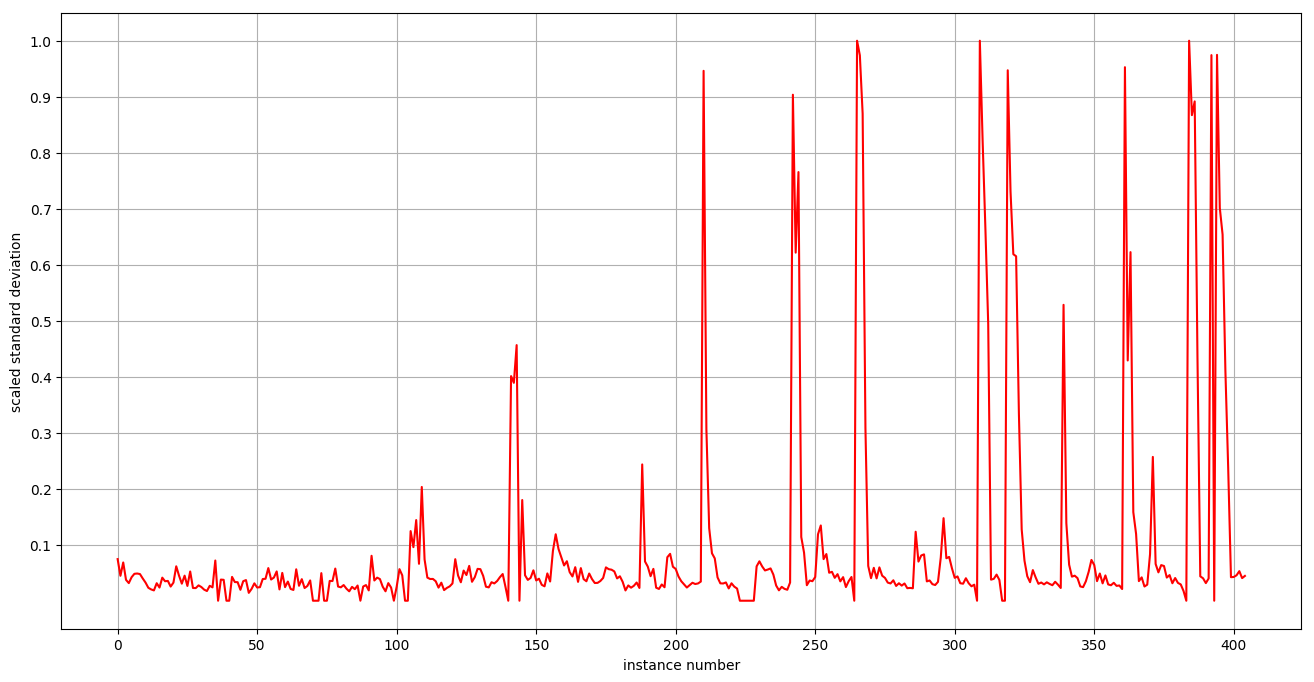
\includegraphics[scale=0.35]{pictures/stddev_graph.png}
    \caption{Scaled Standard Deviation for each Instance}
    \label{fig:stddevperinstance}
\end{figure}

From the graph, it can be seen that most of the instances have a scaled standard deviation of less than $0.1$, which speaks good about the robustness of the algorithm when looking at its independent behaviour from the random numbers given to it. It is worth noting that the occasional spikes, like on the last $13$ instances, is due to the problem mentioned before, that for some instances many solutions were scrapped in the tour Greedy Randomized Construction phase of the algorithm, leaving less solutions built in total and thus less variance between solutions. This is specially true for instances like ``$100-180-15-8\text{.ophs}$'' from ``SET$5\_15-8$'', where $3914$ iterations from the $5000$ ran produced no viable solutions.
